\section{Thuật toán Morriss-Pratt}
\subsection{Đặc điểm chính}


Thuật toán Morris-Pratt là một trong những thuật toán đối sánh mẫu kinh điển, được đề xuất bởi James H. Morris và Vaughan R. Pratt vào năm 1970. Thuật toán được xây dựng nhằm cải thiện hiệu năng của phương pháp đối sánh tuần tự (Brute Force) bằng cách tránh việc so sánh lại các ký tự đã được kiểm tra trước đó.

Ý tưởng cốt lõi của thuật toán là sử dụng thông tin thu được từ các lần khớp trước để xác định vị trí dịch chuyển tiếp theo của mẫu mà không cần quay lui trên văn bản. Để thực hiện điều này, thuật toán xây dựng một bảng tiền xử lý, thường được gọi là bảng thất bại (failure function) hoặc bảng biên (border table), cho biết độ dài tiền tố dài nhất của mẫu đồng thời cũng là hậu tố của chuỗi con đang xét.

Trong quá trình tìm kiếm, khi xảy ra sai khớp, thuật toán không dịch mẫu từng ký tự như phương pháp vét cạn mà sử dụng bảng tiền xử lý để xác định trạng thái khớp phù hợp tiếp theo. Nhờ đó, số lượng phép so sánh được giảm đáng kể.

Thuật toán Morris-Pratt có các đặc điểm chính như sau:

\begin{itemize}
    \item Thực hiện quá trình so sánh từ trái sang phải.
    
    \item Pha tiền xử lý có độ phức tạp thời gian và không gian là \(O(m)\), với \(m\) là độ dài mẫu.
    
    \item Pha tìm kiếm có độ phức tạp thời gian \(O(n + m)\), không phụ thuộc vào kích thước bảng chữ cái.
    
    \item Thực hiện nhiều nhất \(2n - 1\) phép so sánh ký tự trong quá trình quét văn bản.
    
    \item Độ trễ (delay) được chặn trên bởi \(m\).
\end{itemize}

\subsection{Mô tả thuật toán}
Thuật toán Morris-Pratt được xây dựng dựa trên sự phân tích chi tiết thuật toán Brute Force, đặc biệt tập trung vào cách mà thuật toán này chưa tận dụng hiệu quả các thông tin thu được trong quá trình quét văn bản.

Khi phân tích chi tiết thuật toán Brute Force, có thể nhận thấy rằng độ dài dịch chuyển của mẫu có thể được cải thiện đồng thời lưu lại các phần của văn bản đã khớp với mẫu. Nhờ đó, số phép so sánh giữa các ký tự của mẫu và văn bản được giảm đáng kể, góp phần nâng cao tốc độ tìm kiếm.

Xét một lần thử đối sánh tại vị trí bắt đầu \(j\) trên chuỗi văn bản \(y\), tức là khi cửa sổ đối sánh được đặt trên đoạn \(y[j \dots j+m-1]\). Giả sử phép sai khớp đầu tiên xảy ra giữa \(x[i]\) và \(y[i+j]\), với \(0 < i < m\). Khi đó, ta có \(x[0 \dots i-1] = y[j \dots i+j-1] = u\) và \(a = x[i] \neq y[i+j] = b\). Nói cách khác, \(u\) là đoạn tiền tố của mẫu đã khớp hoàn toàn với đoạn tương ứng trong văn bản trước khi xảy ra sai khớp.

Khi thực hiện dịch chuyển mẫu, có thể kỳ vọng rằng một tiền tố \(v\) của mẫu sẽ khớp với một hậu tố của đoạn \(u\) trong văn bản. Tiền tố dài nhất thỏa mãn điều kiện này được gọi là biên (border) của \(u\), tức là chuỗi xuất hiện đồng thời ở cả đầu và cuối của \(u\). Từ đó, định nghĩa \(mpNext[i]\) là độ dài của biên dài nhất của \(x[0 \dots i-1]\), với \(0 < i \leq m\). Khi đó, sau mỗi lần dịch chuyển, quá trình so sánh có thể tiếp tục giữa ký tự \(c = x[mpNext[i]]\) và \(y[i+j] = b\) mà không bỏ sót bất kỳ lần xuất hiện nào của \(x\) trong \(y\), đồng thời tránh việc quay lui trên văn bản. Giá trị \(mpNext[0]\) được gán bằng \(-1\).

\begin{figure}[H]
    \centering
    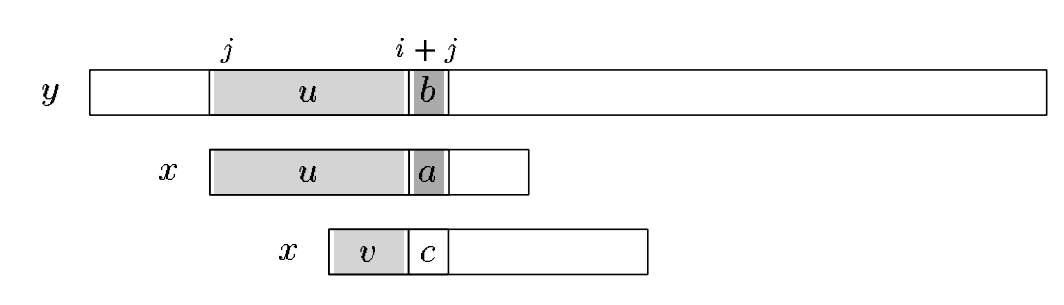
\includegraphics[width=10cm]{Images/mp_1.png}
    \caption{Minh họa bảng mpNext trong thuật toán Morris-Pratt}
    \label{fig:morris-pratt-mpnext}
\end{figure}

Bảng \texttt{mpNext} có thể được tính trước pha tìm kiếm với độ phức tạp thời gian và không gian \(O(m)\) bằng cách áp dụng chính thuật toán tìm kiếm lên mẫu, xem như \(x = y\).

Khi đó, pha tìm kiếm có thể được thực hiện với độ phức tạp thời gian \(O(m+n)\). Trong quá trình tìm kiếm, thuật toán Morris-Pratt thực hiện nhiều nhất \(2n - 1\) phép so sánh ký tự trên văn bản. Độ trễ của thuật toán (số phép so sánh tối đa đối với một ký tự văn bản) được chặn trên bởi \(m\).

\subsection{Cài đặt bằng C++}
\begin{verbatim}
#include <iostream>
#include <vector>
#include <string>

using namespace std;

vector<int> computeMPNext(const string& pattern) {
    int m = pattern.length();

    vector<int> mpNext(m + 1);

    int i = 0;
    int j = -1;

    mpNext[0] = -1;

    while (i < m) {
        while (j > -1 && pattern[i] != pattern[j]) {
            j = mpNext[j];
        }

        ++i;
        ++j;

        mpNext[i] = j;
    }

    return mpNext;
}

vector<int> morrisPratt(const string& pattern, const string& text) {
    int m = pattern.length();
    int n = text.length();

    vector<int> mpNext = computeMPNext(pattern);

    vector<int> occurrences;

    int i = 0;
    int j = 0;

    while (j < n) {
        while (i > -1 && pattern[i] != text[j]) {
            i = mpNext[i];
        }

        ++i;
        ++j;

        if (i >= m) {
            occurrences.push_back(j - i);
            i = mpNext[i];
        }
    }

    return occurrences;
}

int main() {
    string text = "ababcabcabababd";
    string pattern = "ababd";

    vector<int> result = morrisPratt(pattern, text);

    for (int pos : result) {
        cout << "Pattern found at position: " << pos << endl;
    }

    return 0;
}
\end{verbatim}

\subsection{Kiểm nghiệm thuật toán}

\begin{figure}[H]
    \centering
    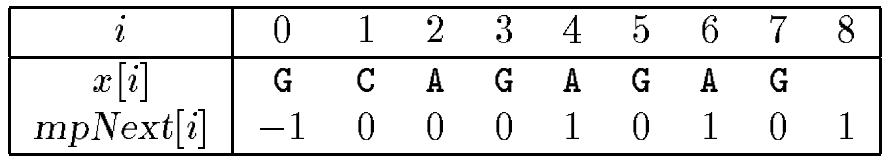
\includegraphics[width=10cm]{Images/2026-05-15-10-04-29.png}
    \caption{Kết quả kiểm nghiệm thuật toán Morris-Pratt}
    \label{fig:morris-pratt-test-overview}
\end{figure}

\textbf{Pha tìm kiếm}
Lần 1:

\begin{figure}[H]
    \centering
    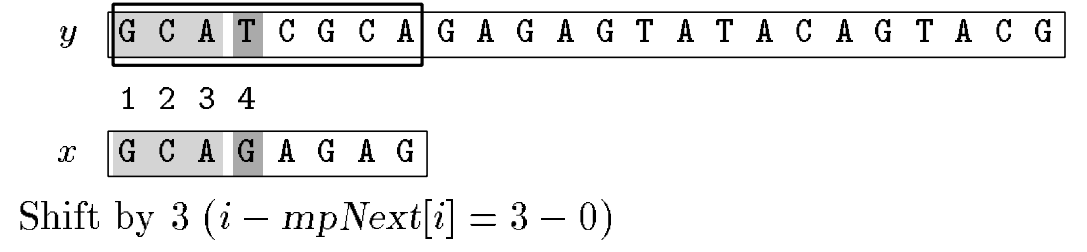
\includegraphics[width=10cm]{Images/2026-05-15-10-08-22.png}
    \caption{Bước 1 trong quá trình thực hiện thuật toán Morris-Pratt}
    \label{fig:morris-pratt-step-1}
\end{figure}

Lần 2:

\begin{figure}[H]
    \centering
    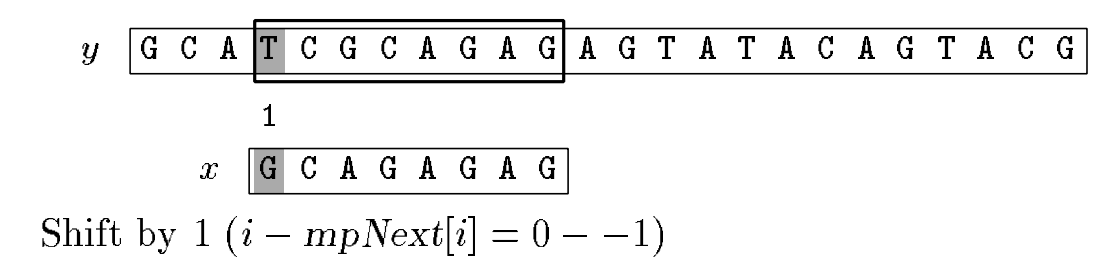
\includegraphics[width=10cm]{Images/2026-05-15-10-08-56.png}
    \caption{Bước 2 trong quá trình thực hiện thuật toán Morris-Pratt}
    \label{fig:morris-pratt-step-2}
\end{figure}

Lần 3:

\begin{figure}[H]
    \centering
    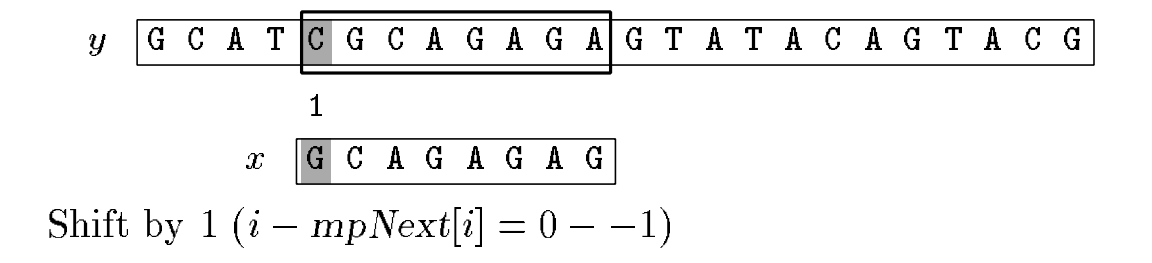
\includegraphics[width=10cm]{Images/2026-05-15-10-09-18.png}
    \caption{Bước 3 trong quá trình thực hiện thuật toán Morris-Pratt}
    \label{fig:morris-pratt-step-3}
\end{figure}

Lần 4:

\begin{figure}[H]
    \centering
    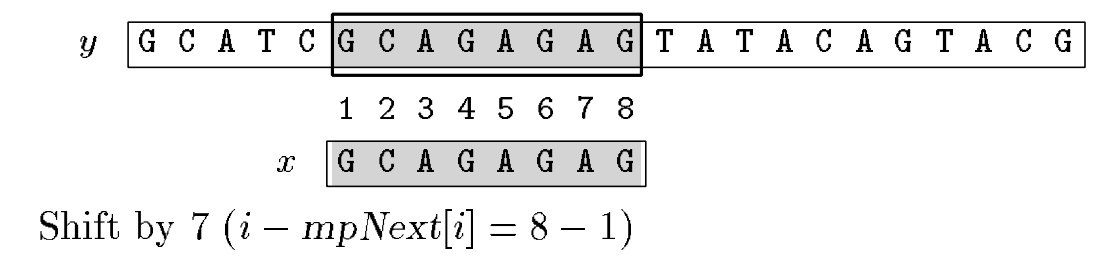
\includegraphics[width=10cm]{Images/2026-05-15-10-09-35.png}
    \caption{Bước 4 trong quá trình thực hiện thuật toán Morris-Pratt}
    \label{fig:morris-pratt-step-4}
\end{figure}

Lần 5:

\begin{figure}[H]
    \centering
    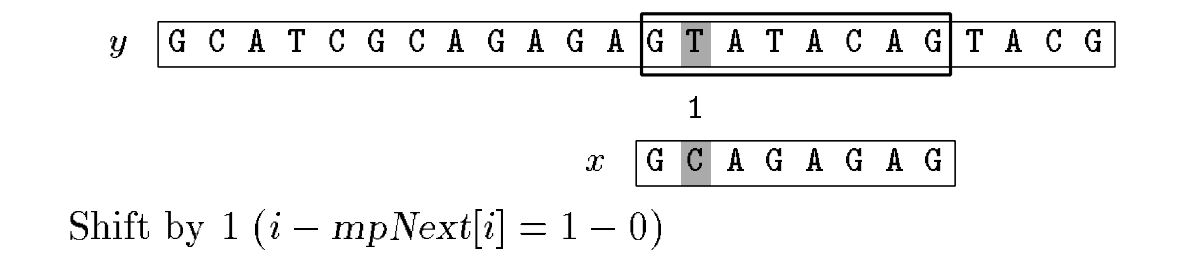
\includegraphics[width=10cm]{Images/2026-05-15-10-09-52.png}
    \caption{Bước 5 trong quá trình thực hiện thuật toán Morris-Pratt}
    \label{fig:morris-pratt-step-5}
\end{figure}

Lần 6:

\begin{figure}[H]
    \centering
    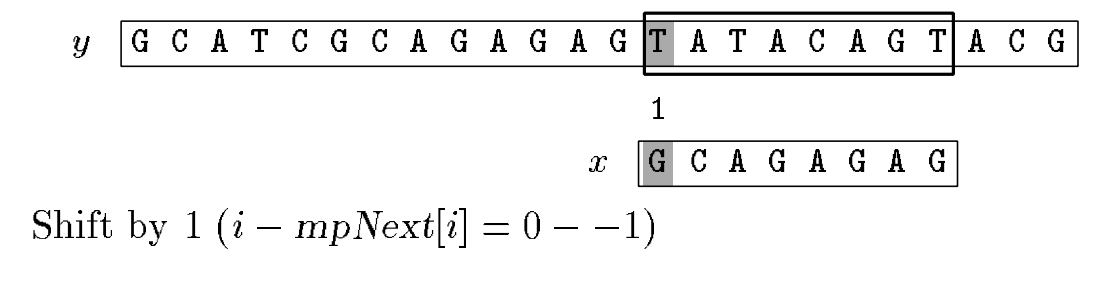
\includegraphics[width=10cm]{Images/2026-05-15-10-10-15.png}
    \caption{Bước 6 trong quá trình thực hiện thuật toán Morris-Pratt}
    \label{fig:morris-pratt-step-6}
\end{figure}

Lần 7:

\begin{figure}[H]
    \centering
    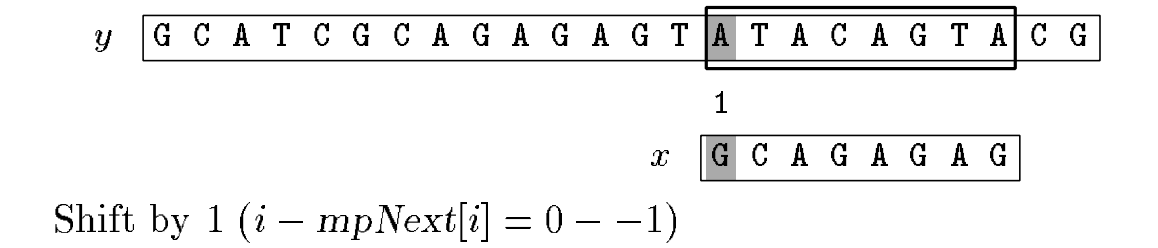
\includegraphics[width=10cm]{Images/2026-05-15-10-10-33.png}
    \caption{Bước 7 trong quá trình thực hiện thuật toán Morris-Pratt}
    \label{fig:morris-pratt-step-7}
\end{figure}

Lần 8:

\begin{figure}[H]
    \centering
    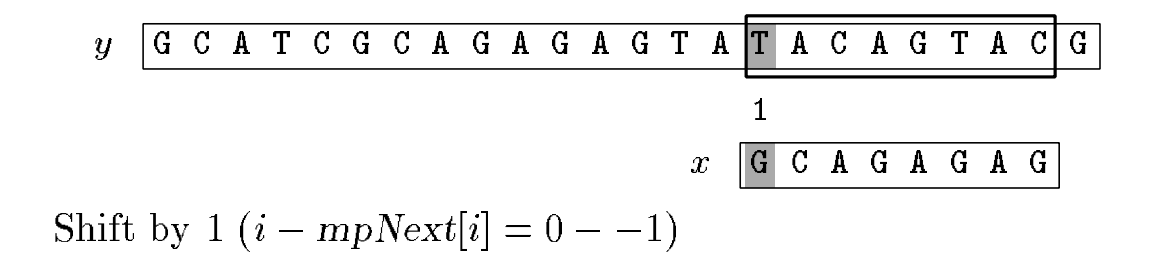
\includegraphics[width=10cm]{Images/2026-05-15-10-10-49.png}
    \caption{Bước 8 trong quá trình thực hiện thuật toán Morris-Pratt}
    \label{fig:morris-pratt-step-8}
\end{figure}

Lần 9:

\begin{figure}[H]
    \centering
    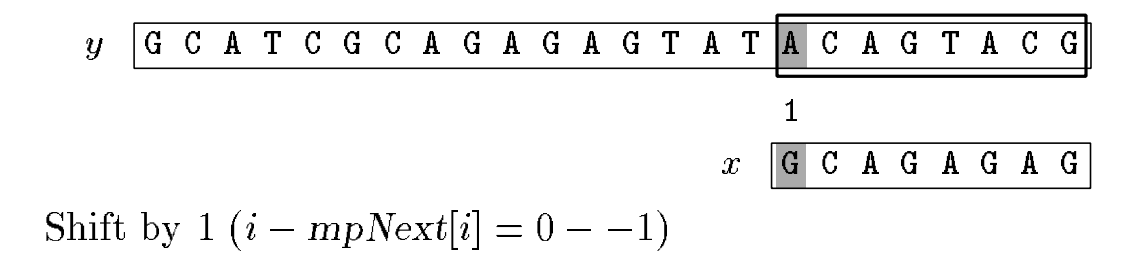
\includegraphics[width=10cm]{Images/2026-05-15-10-11-20.png}
    \caption{Bước 9 trong quá trình thực hiện thuật toán Morris-Pratt}
    \label{fig:morris-pratt-step-9}
\end{figure}

Thuật toán Morris-Pratt thực hiện 19 lần so khớp chuỗi trong ví dụ trên.